\documentclass{article}
\usepackage[utf8]{ inputenc }
\usepackage{ graphicx }
\graphicspath{ {img/} }
\usepackage{ geometry}
\geometry{legalpaper, margin=1.3in}
\usepackage{ bbm }
\usepackage{ braket }
\usepackage{ mathrsfs }
\usepackage{ amssymb }
\usepackage{ mathtools }
\usepackage{ amsfonts }
\usepackage{ caption }
\usepackage{ enumitem }
\usepackage{ tikz }
\usetikzlibrary{ quantikz, arrows,  }
\usepackage[hidelinks]{ hyperref }
\newtheorem{theorem}{Theorem}
\newtheorem{lemma}{Lemma}

\usepackage{ fancyhdr }
\pagestyle{fancy}
\fancyhf{}
\fancyhead[LOE]{\leftmark}
\fancyfoot[COE]{\thepage}

% = with "def" above.
\newcommand\eqdef{\mathrel{\overset{\makebox[0pt]{\mbox{\normalfont\tiny\sffamily
def}}}{=}}}
% = with "goal" above.
\newcommand\eqgoal{\mathrel{\overset{\makebox[0pt]{\mbox{\normalfont\tiny\sffamily
goal}}}{=}}}
% kind of small matrices but not optimal.
\newcommand{\colvec}[2][.8]{%
  \scalebox{#1}{%
    \renewcommand{\arraystretch}{.7}%
    $\begin{bmatrix}#2\end{bmatrix}$%
  }
}
\newcommand{\neswarrow}{\mathrel{\text{$\nearrow$\llap{$\swarrow$}}}}

\title{qk4cs}
\author{}
\date{2021/2022}

\begin{document}

\begin{titlepage}
\begin{center}

\textsc{\LARGE Sorbonne Universite} \\[1cm]
\textsc{\LARGE Master 1 - Quantum Information} \\[1cm]
\textsc{\Large 2021/2022} \\[7cm]


{\huge \bfseries Lecture notes} \\[0.5cm]
{\huge \bfseries -} \\[0.5cm]
{\huge \bfseries Quantum Kinematic} \\[4cm]
\vfill

\includegraphics[scale=0.7]{su.png}

\end{center}
\end{titlepage}

\tableofcontents

\newpage

\section{Introduction}
Physical system which has $d \in \mathbbm{N}$ possible distinguishable states.
Its physical state $\ket{\psi} \in \mathscr{H}$, the Hilbert space
$\mathbbm{C}^d$.

\begin{equation}
    \ket{\psi} = \begin{bmatrix} \psi_1\\ \psi_2 \\ \vdots \\ \psi_d\end{bmatrix}
    \text{ and } \forall i, \psi_i \in \mathbbm{C}.
\end{equation}


\noindent
The result of the measurement in the computational basis on $\ket{\psi}$ is $i
\in [1, \cdots, d]$ with probability $|\psi_i|^2$. \\ \noindent And
$\sum_{i=1}^d |\psi_i|^2 = \braket{\psi|\psi} = 1$: the state is normalized.

\subsection{Dirac notation}

\begin{itemize}[label=-]

\item Ket:
\begin{equation}
\ket{\psi} = \begin{bmatrix} \psi_1\\ \vdots \\ \psi_d\end{bmatrix} = \psi_1 \ket{1} + \cdots + \psi_d\ket{d} = \sum_{i=1}^d \psi_i\ket{i}
\end{equation}
\item Bra:
\begin{equation}
\bra{\psi} = \ket{\psi}^\dagger = \ket{\psi^*}^T
\end{equation}
\item Braket:
\begin{equation}
\braket{\psi|\varphi}
= \begin{bmatrix} \psi_1^* \cdots \psi_d^*\end{bmatrix} \begin{bmatrix} \varphi_1\\ \vdots \\ \varphi_d\end{bmatrix}
= \psi_1^*\varphi_1 + \cdots + \psi_d^*\varphi_d
\end{equation}
$\braket{\psi|\varphi} $ is the hermitian product of $\psi$ and $\varphi$.
\end{itemize}

\subsection{Measurement in a basis \texorpdfstring{$B$}{Lg}} $B$ is an
orthonormal basis : $B := \{\ket{b_i}\}_{i=1}^d$, with the following properties:
\begin{equation}
    \begin{aligned}
        \forall i \braket{b_i|b_i} = \delta_{i, j} & \text{ \textit{ (orthonormality)}} \\
        \sum_{i=1}^d\ket{b_i}\bra{b_j} = I & \textit{ (completeness)}
    \end{aligned}
\end{equation}

\begin{figure}[h]
\centering
\begin{quantikz}
    \lstick{$\ket{\psi}$} & \qw & \meter{$B$} & \qw \arrow[r] & \rstick{$i$} \qw
\end{quantikz}
\caption{Circuit representation of the measurement of the state $\ket{\psi}$\\
in the basis $B$.}
\end{figure}

\noindent
The probability of the output of a measurement is given by the following formula
:
\begin{equation}
    \mathbbm{P}(out=\ket{b_i}) = |\braket{b_i|\psi}|^2
\end{equation}
The physical object is projected into the state $\ket{b_i}$, this is physically
called the "wave packet reduction".

\subsubsection*{Qubit}
\begin{equation}
    \ket{0}= \begin{bmatrix} 1 \\ 0 \end{bmatrix}
    \hspace{1.2in}
    \ket{1}= \begin{bmatrix} 0 \\ 1 \end{bmatrix}
\end{equation}
\begin{equation}
    \ket{+} = \frac{1}{\sqrt2}(|0\rangle + |1\rangle)
    \hspace{0.7in}
    \ket{-}= \frac{1}{\sqrt2}(|0\rangle - |1\rangle)
\end{equation}

\subsubsection*{Measurement in the basis \texorpdfstring{$\{\ket{\pm}\}$}{Lg}}
\begin{figure}[h]
\centering
\begin{quantikz}
    \lstick{$\ket{0}$} & \qw & \meter{$\pm$} & \qw \arrow[r] & \rstick{$
        \begin{cases}
            +, & \text{w.p. $|\braket{+|0}|^2=\frac{1}{2}$}\\
            -, & \text{w.p. $|\braket{-|0}|^2=\frac{1}{2}$} \end{cases}$} \qw
\end{quantikz}
\caption{Measure of the state $\ket{0}$ in the basis $\ket{\pm}$}
\end{figure}

\subsection{Wiesner's Quantum Money}
Based on the conjugate coding.

\begin{itemize}[label=-]
    \item \texttt{bills}:
    \begin{itemize}
        \item serial number
        \item a set of random qubit $E_r \in \{\ket{0}, \ket{1}, \ket{+},
        \ket{-}\}^n$
        \item \texttt{mint} knows $\{\text{Serial Number}+\text{Random}\}$,
        sends it to the bank.
    \end{itemize}
    \item \texttt{Mint}: makes the bill, and gives it to the forger.
    \item \texttt{Forger}: tries to copy the bill, and spends the two to the
    bank.
    \item \texttt{Bank}: should accept the true one, reject the fake.
\end{itemize}

\begin{table}[h]
    \centering
    \begin{tabular}{c|c|c|c}
    \texttt{mint} & \texttt{forger} basis & \texttt{forger} m. & \texttt{bank}
    m. \\\hline
    $\ket{0}$ & $\{\ket{0}, \ket{1}\}$ & $\ket{0}$ & $\ket{0} $\\
    $\ket{0}$ & $\{\ket{\pm}\}$ & $\begin{cases} \ket{+}, & \text{w.p.
    $\frac{1}{2}$}\\
        \ket{-}, & \text{w.p. $\frac{1}{2}$} \end{cases}$ & $\begin{cases}
    \ket{0}, & \text{w.p. $\frac{1}{2}$}\\
        \ket{1}, & \text{w.p. $\frac{1}{2}$} \end{cases}$
    \end{tabular}
\end{table}

We therefore deduce that
\begin{equation}
\mathbbm{P}(\text{get caugth})= 1-(1-\frac{1}{4})^n = 1-(\frac{1}{4})^n
\end{equation}

\subsection{Bennett and Brassard Quantum Key Exchange: BB84}
Goal: Alice and Bob $\rightarrow$ share a secret bit string , Eve does not know
anything. \\
Settings: Alice and Bob share a quantum channel and an authenticated classical
channel. \\\noindent Steps:
\begin{enumerate}
    \item Alice prepares $n$ qubits $E_r \in \{\ket{0}, \ket{1}, \ket{+},
    \ket{-}\}^n$, and she sends them to Bob
    \item Bob receives . He measures them in the basis $\{B_{0,1}, B_{+,-}\}$
    \item They use the public classical channel to compare the basis Bob used.
    They throw away the \textit{bad basis} qubits.
    \item Alice and Bob sample the data and compare the error rate $e$. If
        $e=0$, they keep the key; if $e = 25\%$, Eve knows the key.
\end{enumerate}
What if $0 < e < 25$ ? Eve knows a part of the key.
\section{Unitary transformation}
A transformation is an isolated system, and it is reversible. \\
Let $T$ to be a transformation.
\begin{equation}
    \braket{T(\ket{\psi})|T(\ket{\psi})}=\braket{\psi|\psi}
\end{equation}
$T$ is linear.
\begin{equation}
    T(\alpha\ket{\psi} + \beta\ket{\varphi}) = \alpha T(\ket{\psi}) + \beta T(\ket{\varphi})
\end{equation}
$T$ acts like an unitary operator. $T$ corresponds to a complex matrix $U$:
$T(\ket{\varphi}) = U\ket{\varphi}$, $U \in \mathbbm{C}^{n \times n}$, such that
$U^\dagger U= Id$.
In the basis $\{\ket{i}\}_{i=0}^n$, which is the computational basis,
$\braket{T(\ket{\psi})|T(\ket{\psi})} = \braket{i|j} = \delta_{i,j}$
\\
\\
We have :
\begin{itemize}[label=-]
    \item measurement in computational basis
    \item a machine making arbitrary unitary $U$
\end{itemize}
Let's build a measurement in basis $\{\ket{b_i}\}_i$

\begin{figure}[h]
    \centering
    \begin{quantikz}
        \lstick{$\ket{\psi}$} & \qw & \gate{U} & \phase{U\ket{\psi}}&\meter{} &
        \qw \arrow[r] & \rstick{$i$} \qw
    \end{quantikz}
    \caption{Circuit representation of the measurement unitary exptected behavior}
\end{figure}
\begin{equation}
    \mathbbm{P}(i) \eqdef |\braket{i|U|\psi}|^2 \eqgoal |\braket{b_i|\psi}|^2 \quad \forall \psi
\end{equation}
We want $\bra{i}U=\bra{b_i} \Leftrightarrow U^\dagger\ket{i} = \ket{b_i}
\Leftrightarrow U = \sum_i \ket{i}\bra{b_i}$.
\\
\\\noindent Indeed, if  $U = \sum_i \ket{i}\bra{b_i}$ then $U^\dagger = \sum_i
\ket{b_i}\bra{i}$, that implies $U^\dagger \ket{i} =
\big(\sum_j\ket{b_j}\underbrace{\bra{j}\big)\ket{i}}_{\delta_{i,j}} = \ket{i}$.
\\
\\\noindent
Is $U$ an unitary ?

\begin{equation}
    \begin{aligned}
        U^\dagger U &= \Big(\sum_i \ket{b_i}\bra{i}\Big)\Big(\sum_j\ket{j}\bra{b_j}\Big) \\
        &= \sum_{i, j}\ket{b_i}\braket{i|j}\bra{b_j} \\
        &= \sum_i \ket{b_i}\bra{b_i} \\
        &= Id & U \text{ is an unitary. }
    \end{aligned}
\end{equation}

\section{Composition of systems}
Let $A \in \mathscr{H}_A = \mathbbm{C}^{d_A}$ and $B \in \mathscr{H}_B =
\mathbbm{C}^{d_B}$ to be two systems in their respective vector spaces. Then we
can construct the space
\begin{equation}
    \mathscr{H}_{AB} = \mathscr{H}_A \otimes \mathscr{H}_B
\end{equation}
Its orthonormal basis is $\{\ket{ij}_{AB}\}_{i, j}$, and
\begin{equation}
    \text{dim}\mathscr{H}_{AB} = \text{dim}\mathscr{H}_A \cdot \text{dim}\mathscr{H}_B
\end{equation}
\\\noindent If $\ket{\alpha} = \sum_i\alpha_i\ket{i}_A$ and $\ket{\beta} =
\sum_i\beta_i\ket{i}_B$, then
\begin{equation}
    \ket{\varphi}_{AB}=\ket{\alpha} \otimes \ket{\beta} = \sum_{i,j}\alpha_i\beta_j\ket{i}_A\ket{j}_B
\end{equation}

and $\ket{\varphi}_{AB} \in \mathscr{H}_{AB}$. $\ket{\varphi}_{AB}$ is a joint state
of systems $A$ and $B$. \\\noindent The inner product between two basis states
can be defined as
\begin{equation}
    \braket{i,j|k,l}=\braket{i|k}_A\braket{j|l}_B = \delta_{ik}\delta_{jl}
\end{equation}
\\\noindent The most general state in the space $\mathscr{H}_{AB}$ can be
written
\begin{equation}
    \ket{\psi} = \alpha \ket{00} + \beta \ket{01} + \gamma \ket{10} + \delta \ket{11}
\end{equation}
with the usual condition for $\ket{\psi}$ to be normalized:
\begin{equation}
    |\alpha|^2+|\beta|^2+|\gamma|^2+|\delta|^2 = 1
\end{equation}
\\\noindent Not all states of $\mathscr{H}_{AB}$ are separable into one state of
$\mathscr{H}_{A}$ and one state of $\mathscr{H}_{B}$

For example : $\frac{1}{\sqrt{2}}(\ket{00} + \ket{11}) \in \mathscr{H}_{AB}$,
but $\nexists \ket{\alpha}\in \mathscr{H}_A, \ket{\beta}\in \mathscr{H}_B$, such
that \\\noindent $\ket{\alpha}\otimes\ket{\beta} = \frac{1}{\sqrt{2}}(\ket{00} +
\ket{11})$.

Necessary condition on the coefficients $(\alpha, \beta, \gamma, \delta)$ of a
state to be separable:
\begin{equation}
    \alpha\delta = \beta\gamma
\end{equation}

\subsection{Partial measurement}
\subsubsection*{Case of the 2-qubits state}
Let $\ket{\psi} = \alpha \ket{00} + \beta \ket{01} + \delta \ket{10} + \gamma
\ket{11}$. If we consider not the measurement of the two qubits but only the
measurement of, for this example, the first qubit, the probablilies of having
$0$ or $1$ as outcome are simply given by:
\begin{equation}
    \begin{aligned}
        \mathbb{P}(\ket{0}) & = |\alpha|^2 + |\beta|^2 \\
        \mathbb{P}(\ket{1}) & = |\delta|^2 + |\gamma|^2
    \end{aligned}
\end{equation}
We can rewrite $\ket{\psi} = \ket{0}(\alpha \ket{0} + \beta \ket{1}) +
\ket{1}(\delta \ket{0} + \gamma \ket{1})$, hence we deduce that the final state
after the measurement is $\frac{\alpha \ket{0} + \beta \ket{1}}{\sqrt{|\alpha|^2
+ |\beta|^2}}$ if the measurement outcome was $\ket{0}$, and
$\frac{\delta \ket{0} + \gamma \ket{1}}{\sqrt{ |\delta|^2 +
|\gamma|^2}}$ if the measurement outcome was $\ket{1}$.

As a matter of intution, imagine that we separate both qubits of
the system by a long distance, then acting on the qubit we measure should not do
anything on the other, hence we juste need to sum the probabilities.

\subsection{No cloning theorem}
\begin{theorem}
    There is no unitary $U$ such that $\forall \ket{\psi} \in \mathscr{H},
    U\ket{\psi} = \ket{\psi} \otimes \ket{\psi} \in \mathscr{H} \otimes
    \mathscr{H}$.
\end{theorem}
\paragraph{Proof: }
Suppose there exists a such unitary U, then U is a cloning operator.
\begin{equation}
    \begin{aligned}
        \forall \ket{\psi}, U\ket{\psi} \eqdef \ket{\psi}\ket{\psi}
    \end{aligned}
\end{equation}

By computing the application of $U$ on the state $\ket{+}$, we get on the one
hand, by linearity of unitaries.
\begin{equation}
    U(\frac{\ket{0}+\ket{1}}{\sqrt{2}}) = \frac{\ket{00}+\ket{11}}{\sqrt{2}}
\end{equation}
\\
and on the other hand, by definition of the operator behavior
\begin{equation}
    U(\frac{\ket{0}+\ket{1}}{\sqrt{2}}) = \frac{\ket{0}+\ket{1}}{\sqrt{2}}
    \otimes \frac{\ket{0}+\ket{1}}{\sqrt{2}}
    =\frac{1}{2}(\ket{00}+\ket{01}+\ket{10}+\ket{11})
\end{equation}
\\
which is a contradiction. Then such a $U$ operator can not exist.

\subsection{Superdense coding}
\textit{Superdense coding} involves two parties, \texttt{Alice} and
\texttt{Bob}. The protocol allows \texttt{Alice} and \texttt{Bob} to share two
bits of information by exchanging just one qubit. Basically, \texttt{Alice} is
in possession of two classical bits of information, which she wishes to send to
\texttt{Bob}.
Suppose \texttt{Alice} and \texttt{Bob} initially share a pair of qubits in the
entangled state
\begin{equation}
    \ket{\psi} = \frac{\ket{00} + \ket{11}}{\sqrt{2}}
\end{equation}
Here is the procedure.

\begin{table}[h]
    \centering
    \begin{tabular}{c|c|c}
    The state \texttt{Alice} wants to send & The gate she applies & The states
    after \\
    $\ket{00}$ & $I$ & $\frac{\ket{00} + \ket{11}}{\sqrt{2}} = \ket{\varphi^+}$  \\
    $\ket{01}$ & $Z$ & $\frac{\ket{00} - \ket{11}}{\sqrt{2}} = \ket{\varphi^-}$ \\
    $\ket{10}$ & $X$ & $\frac{\ket{10} + \ket{01}}{\sqrt{2}} = \ket{\psi^+}$ \\
    $\ket{11}$ & $Y$ & $\frac{\ket{01} - \ket{10}}{\sqrt{2}} = \ket{\psi^-}$
    \end{tabular}
\end{table}
\texttt{Alice} sends her qubit to \texttt{Bob} and he measures the resulting pair
in the base \\
$\{\ket{\varphi^+}, \ket{\varphi^-},\ket{\psi^+}, \ket{\psi^-}\}$. This is indeed a
basis, and its name is the \textit{Bell basis}, and the states are called the
\textit{Bell states}.


\subsection{Quantum teleportation}
%TODO: comes from on the the firsts TD

\section{Measurements}
\subsection{Projective measurement}
A projective measurement is described by an observable, a Hermitian operator.
They are defined by a set of projectors $\{\Pi_j\}_{j=1}^k, k \leq d$.\\
Projectors properties:
\begin{equation}
    \forall j, \Pi_j^2 = \Pi_j \qquad \Pi_j\Pi_i = \delta_{i,j}\Pi_j
\end{equation}
\\\noindent A projector is defined as follows:
\begin{equation}
    \Pi_j = \sum_{l=1}^{d_j}\ket{l_l^j}\bra{l_l^j}
\end{equation}
Upon measuring the state $\ket{\psi}$, the probability of getting result $j$ is
given by
\begin{equation}
    \braket{\psi|\Pi_j|\psi} = \| \Pi_j\ket{\psi}\|^2
\end{equation}
Given that outcome $j$ occured, the state of the quantum system immediately
after the measurement is
\begin{equation}
    \frac{\Pi_j\ket{\psi}}{\| \Pi_j\ket{\psi}\|^2}
\end{equation}

\subsection{Observables}
Observables correspond to physical quantities, with values in $\mathbbm{R}$.
They are well defined in a basis $\{\ket{b_i}\}_i$ (i.e $\forall \ket{b_i},
\exists a_i \in \mathbbm{R})$

\paragraph{Note :} $\alpha\ket{b_1} + \beta\ket{b_2}$ has \textbf{not always} a
well defined value. \\
\\
An observable is defined as follow:
\begin{equation}
    O \eqdef \sum_i o_i \underbrace{\ket{b_i}\bra{b_i}}_{\text{projector on $\ket{b_i}$}}
    = \sum_j o_j \Pi_j
\end{equation}
$O$ is diagonalizable by definition and $O^\dagger = O$: $O$ is hermitian.
\begin{equation}
\text{Shape of $O$ } :
\begin{pmatrix}
    o_1 & 0 & \cdots & 0 \\
    0 & o_2 & \cdots & \vdots \\
    \vdots  & \vdots  & \ddots & \vdots  \\
    0 & \cdots & \cdots & a_d
\end{pmatrix}
\end{equation}
The probability of getting the result $i$ by measuring $O$ on a state
$\ket{\psi}$ is
\begin{equation}
\mathbbm{P}(i)=\braket{\psi|\Pi_i|\psi}
\end{equation}
\subsubsection*{Expectation value and standard deviation}
The expectation value of $O$, written $\langle O\rangle$, is given by
\begin{equation}
    \begin{aligned}
        \langle O\rangle
            & = \sum_i o_i \mathbbm{P}(i\ket{\psi}) \\
            & = \sum_i o_i \|\Pi_i\ket{\psi}\|^2 \\
            & = \sum_i o_i \braket{\psi|\Pi_i|\psi} \\
            & = \bra{\psi}\sum_i o_i \Pi_i \ket{\psi} \\
            & = \braket{\psi | O |\psi}
    \end{aligned}
\end{equation}
From this formula for the expectation value follows a formula for the standard
deviation associated to the observation of $O$
\begin{equation}
    \Delta^2 O = \langle(O - \langle O \rangle)^2\rangle = \langle O^2 \rangle - \langle O \rangle^2
\end{equation}

\paragraph{Note:} If $\ket{\psi}$ is an eigenstate of $O$, then $O\ket{\psi} =
\lambda \ket{\psi}$. \\
Hence:
\begin{equation}
    \begin{aligned}
        \braket{O}
            & = \braket{\psi | O | \psi} \\
            & = \braket{\psi | \lambda | \psi} \\
            & = \lambda\braket{\psi|\psi } \\
            & = \lambda
    \end{aligned}
\end{equation}
\\
And:
\begin{equation}
    \begin{aligned}
        O\ket{\psi} = \braket{O} \ket{\psi}
            & \Rightarrow \Delta^2 O = (\lambda^2 - \lambda^2) = 0 \\
            & \Rightarrow \Delta O = 0
    \end{aligned}
\end{equation}

\subsubsection*{Commutators}
A key property of quantum physics is the existence of incompatible measurements:
for any physical property $A$, there exists another physical property $B$ which
is incompatible with $A$. The incompatible means it is physically impossible to
prepare a state $\ket{\psi}$ which gives perfectly predictible outputs for both
measurements $A$ and $B$. Let us first assume $A$ and $B$ to be observables. A
key property of this pair of observable is their commutator
\begin{equation}
    [A,B]:= AB-BA
\end{equation}

If $A$ and $B$ commute (i.e $[A,B]=0 \Leftrightarrow AB = BA$), there exists a
basis such that the result of a measurement of $A$ and a measurement of $B$ are
perfectly defined.

Conversely, if such a basis exists, then $[A,B]=0$

Therefore, if $A$ and $B$ do not commute, they correspond to incompatible
measurements. (The proofs are in the $4^{th}$ tutorial.)

\subsubsection*{The Robertson-Heisenberg uncertainty relation}
This relation evaluates the sharpness of two observables we will call $A$ and
$B$ through the standard deviations $\Delta A$ and $\Delta B$, and the states
that, for any state $\ket{\psi}$ and any observable $A$ and $B$

\begin{equation}
    \Delta A \Delta B \geq \frac{1}{2}\big|\braket{\psi|[A,B]|\psi}\big|
\end{equation}

\subsubsection*{Anti-commutator}
The anti commutator of two observables $A$ and $B$ is defined by
\begin{equation}
    \{A,B\} = AB+BA
\end{equation}

\subsubsection*{Example}
Using the Pauli matrix $\sigma_x = X =
    \begin{bmatrix}
    0 & 1 \\
    1 & 0
    \end{bmatrix}
    = \ket{+}\bra{+} - \ket{-}\bra{-} $. \\\noindent Known results : $X\ket{+} =
    \ket{+}$ and $X\ket{-}=-\ket{-}$. \\\noindent We define
    $\ket{\theta}:=\cos\theta\ket{0}+\sin\theta\ket{1}$ \\\noindent Then
\begin{equation}
    \begin{aligned}
        \langle X \rangle_{\ket{\theta}}
            & = \braket{\theta | X |\theta} \\
            & = [\cos \theta \sin \theta]
                \begin{bmatrix}0 & 1 \\ 1 & 0 \end{bmatrix}
                \begin{bmatrix} \cos \theta\\ sin \theta \end{bmatrix} \\
            & = 2 \sin\theta\cos\theta \\
            & = \sin (2\theta)
    \end{aligned}
\end{equation}


\subsection{Generalized measurements}
A generalized measurement is defined by
\begin{equation}
    \{K_i\}_i \text{ such that } \sum_i K_i^\dagger K_i=Id
\end{equation}
where the $K_i$ are called Kraus Operators. The probability of getting the
result $i$ from a general measurement operator is given by $\mathbbm{P}(i) =
\|K_i\ket{\psi}\|^2$ , and the state of the system just after the measurement is
$K_i\ket{\psi}=\frac{K_i\ket{\psi}}{\|K_i\ket{\psi}\|^2}$

\subsubsection*{Generalized measurement $\rightarrow$ Operator}
If $i \in \{1\}$ then $K_1^\dagger K_1=Id \Rightarrow K_1$ is
unitary.%FIXME: not sure of that.

\subsubsection*{Generalized measurement $\rightarrow$ Set of projectors}
If $K_i := \Pi_i$ then $\sum_i K_i^\dagger K_i = \sum_i \Pi_i^\dagger\Pi_i =
\sum_i \Pi_i = Id$

\subsubsection*{Example}
With probability $p_j$, I measure $\{\Pi_{ij}\}_i \text{ (with } \sum_i \Pi_{ij} = Id)$ and
I measure $U_j$ on the output state.
The probability of getting $ij$ as measurement outcome is given by:
\begin{equation}
    \begin{aligned}
        \mathbbm{P}(ij)
            &= p_j\braket{\psi | \Pi_{ij} U^\dagger U \Pi_{ij} | \psi} \\
            &= p_j\braket{\psi|\Pi_{ij}|\psi}
    \end{aligned}
\end{equation}
\noindent
And the resulting state is
$\dfrac{U\Pi_{ij}\ket{\psi}}{\|\Pi_{ij}\ket{\psi}\|^2}$

\noindent
Let $\{K_{ij} =\sqrt{p_j} U \Pi_{ij}\}_{ij}$, then
\begin{equation}
    \begin{aligned}
        \sum_{ij} K_{ij}^\dagger K_{ij}
            & = \sum_{ij} p_j \Pi_{ij} U^\dagger U \Pi_{ij} \\
            & = \sum_j p_j \sum_i \Pi_{ij} \\
            & = \sum_j p_j \\
            & = Id
    \end{aligned}
\end{equation}
\noindent
Can we associate each set $\{K_i\}_i$ with a $U$ and a $\{\Pi_i\}_i$ ?
\begin{figure}[h]
    \centering
\begin{quantikz}
        \lstick{$\ket{\psi}_I$} & \qw \gategroup[2,steps=5,style={dashed,rounded
        corners,fill=blue!20, inner xsep=2pt},background]{{\sc $\{K_i\}_i$}} &
        \qw & \qw & \gate[2]{U} & \qw\arrow[r] & & \text{ouput $o$} \\
        & & & \lstick{   $\ket{0}_A$} & \qw & \meter{M$\{\ket{i}\}$} & \qw
        \arrow[r] & \text{ }i
    \end{quantikz}
    \caption{Circuit representation of such $U$ and $\{\Pi_i\}_i$. \\
    Note: $\mathscr{H}_A\otimes \mathscr{H}_I =
    \mathscr{H}_O\otimes\mathscr{H}_M$}
\end{figure}
\\\noindent $\forall i,$ the output state of the system is
\begin{equation}
    \label{output-state-kraus}
    (I_o \otimes \ket{i}_M\bra{i})U\ket{\psi}\otimes\ket{0}_A = \ket{i}_M\braket{i|U|0}_A\ket{\psi}_I
\end{equation}
Assume $K_i = _M\braket{i|U|0}_A$. With (\ref{output-state-kraus}), we deduce
that the output state is $K_i\ket{\psi}$, w.p. $\braket{\psi|K_i^\dagger
K_i|\psi}$. Is $\{K_i\}_i$ a valid set of operators ?
\begin{equation}
    \begin{aligned}
        \sum_i K_i^\dagger K_i
        & = \sum_i \big(_A\bra{0}\otimes I_I\big) U^\dagger \big(\ket{i}_M \otimes I_O\big)\big(I_O \otimes
        _M\bra{i}\big)U\big(I_I\otimes \ket{0}_A\big)\\
        & = (_A\bra{0}\otimes I_I)
        \underbrace{U^\dagger (
        \underbrace{
            \underbrace{
                \sum_i \ket{i}_M}_{=I_M}
                    \otimes I_O
            }_{=I_{OM}})
            (I_O \otimes _M\bra{i})
        }_{= I_{OA}}(I_I\otimes \ket{0}_A) \\
        & = (_A\bra{0}\otimes I_I)I_{OA}(I_I\otimes \ket{0}_A) \\
        & = I_O \qquad \text{$\{K_i\}_i$ is a valid set.}
    \end{aligned}
\end{equation}

\subsubsection*{$\{K_i\}_i \rightarrow$ Unitary} Let $U := \sum_i K_i \otimes
\ket{i}_{MA}\bra{0} + \cdots $. The $\cdots$ represents extra terms used to make
$U$ a unitary, but can be neglected in the computation. By tensoring with
$\ket{0}_A$, we obtain
\begin{equation}
    U\ket{\psi}\otimes \ket{0}_A = \sum_i K_i \ket{\psi}\otimes\ket{i}
\end{equation}
And then
\begin{equation}
    \begin{aligned}
        _A\braket{0 |U^\dagger U|0}_A
            & = _A\bra{0}(\sum_i\ket{0}_{AM}\bra{i} K_i^\dagger \cdot \sum_j
            K_j\ket{j}_{AM}\bra{0})\ket{0}_A \\
            & = \underbrace{_A\braket{0|0}_A}_{=1} \cdot \sum_{ij}(_M\bra{i}\otimes
            K_i^\dagger)(\ket{j}_M\otimes K_j) \underbrace{_A\braket{0|0}_A}_{=1} \\
            & = \sum_{ij}\underbrace{\braket{i|j}}_{\delta_{ij}} K_i^\dagger K_j \\
            & = \sum_i K_i^\dagger K_i \\
            & = Id
    \end{aligned}
\end{equation}
\subsection{POVMs}
POVMs means Projective Operator Valued Measure: differently from the projective
measurements, the POVM does not define the post-measurement state.\\
Recall that the probability of getting $i$, when the state is $\ket{\psi}$ is
\begin{equation}
\braket{\psi | K_i^\dagger K_i | \psi}
\end{equation}
Then let $E_i = K_i^\dagger K_i$.\\\noindent POVMs are then defined by the set
$\{E_i\}_i$, such that
\begin{equation}
\sum_i E_i = Id, \quad E_i\geq 0
\end{equation}
$E_i$ is semi-definite positive: $ \forall \psi, \braket{\psi|E_i|\psi} \geq 0$.
This implies that $E_i$ is hermitian, and all its eigenvalues are $\geq 0$.

\subsection{The global phase}\label{global-phase}
\begin{lemma}
The global phase is irrelevant.
\end{lemma}
Of couse, the state $\ket{\psi}$ is different from the state
$e^{i\varphi}\ket{\psi}$, but there is no way to measure the factor
$e^{i\varphi}$.

\paragraph{Proof: }
First, we have
\begin{equation}
    |\braket{\psi|e^{i\varphi}|\psi}|^2 = |e^{i\varphi}|^2 = 1
\end{equation}
Using the generalized measurements $\{K_i\}_i$ such that $\sum_i K_i^\dagger K_i
= Id$ \\\noindent
Then, since $e^i\varphi \in \mathbb{C}$, it commutes with $K_i$:
\begin{equation}
    K_ie^{i\varphi}\ket{\psi} = e^{i\varphi}K_i\ket{\psi}
\end{equation}
\noindent
The phase of the input is the same as the phase of the output. \\\noindent And
\begin{equation}
    \begin{aligned}
        \|K_ie^{i\varphi}\ket{\psi}\|^2_2
            & =\begin{cases}
               \| K_i \ket{\psi} \|_2^2 & =  \sqrt{ \mathbb{P}(i\ket{\psi})} \\
               \|e^{i\varphi} K_i\ket{\psi}\|_2^2 & =  \sqrt{\mathbb{P}(i|e^{i\varphi}\ket{\psi})}
            \end{cases}
    \end{aligned}
\end{equation}
\\\noindent Hence, the global phase is irrelevant, and there is no way to
measure the global phase. \\\noindent However, the relative phase is important
for later computations.
\begin{equation}
    \frac{1}{\sqrt{2}}(\ket{0}+\underbrace{e^{i\varphi}}_{\text{relative phase}}\ket{1})
\end{equation}
For example the $Z$ gates changes the relative phase and $HZH\ket{0} = \ket{1}\neq
HH\ket{0} = \ket{0}$ due to the relatve phase added by $Z$.

\subsection{General quantum state}
\subsubsection*{Number of parameters to describe a quantum state}
Let $\mathscr{H} = \mathbbm{C^d}$ and $\ket{\psi} \in \mathscr{H}: \ket{\psi} =
\sum_{i=0}^d \alpha_i \ket{i}$ , (with $\alpha_i \in \mathbbm{C}$ and $\sum_i
|\alpha_i|^2=1$). If we consider $\alpha_i \in \mathbbm{R}$ is the global phase,
then $2d-2$ real parameters are needed to represent the quantum state.

\subsubsection*{Example}
Qubit in $\mathscr{H}$:
\begin{itemize}[label=-]
    \item $d=2 \rightarrow 2\cdot2-2 = 2$ real parameters : $(\theta, \varphi)$.
    \item $d=3 \rightarrow 4$ real parameters.
\end{itemize}
A quantum state can be written, with the parameters $\theta$ and $\varphi$, as
\begin{equation}
    \ket{\theta, \varphi} = \cos \frac{\theta}{2}\ket{0} + e^{i\varphi}\sin \frac{\theta}{2}\ket{1}
\end{equation}

\section{Bloch sphere}
\begin{figure}[h]
    \centering
    \includegraphics[scale=0.15]{bloch-sphere.png}
    \caption{Graphical representation of a quantum state in the Bloch sphere}
\end{figure}
\noindent
We will denote $\ket{\psi}$ as the vector $\vec{m}$
\begin{equation}
    \begin{aligned}
        \vec{m} & = \begin{bmatrix}
            u \\ v \\ w
        \end{bmatrix} \text{such that } u^2 + v^2 + w^2 = 1
    \end{aligned}
\end{equation}
\text{whose cartesian coordinates are \quad}
\begin{equation}
    \begin{aligned}
        \vec{m} & =
        \begin{bmatrix}
            \label{def-vect-m}
            \sin \theta \cdot \cos \varphi \\
            \sin \theta \cdot \sin \varphi \\
            \cos \theta
        \end{bmatrix}
    \end{aligned}
\end{equation}
Are $\vec{m}$ and $\vec{-m}$ orthogonal ?
\begin{equation}
    \label{m-m-orthogonal}
    \begin{aligned}
        \braket{m|-m}
            & = \braket{\theta,\varphi|\pi-\theta,\varphi+\pi[2\pi]} \\
            & = \Big(\cos\frac{\theta}{2}\bra{0}+e^{i\varphi}\sin\frac{\theta}{2}\bra{1}\Big)
                \Big(\underbrace{\cos(\frac{\pi}{2}-\frac{\theta}{2})}_{\sin\frac{\theta}{2}}
                \ket{0}+e^{i(\varphi+\pi)}
                \underbrace{\sin(\frac{\pi}{2}-\frac{\theta}{2})}_{
                \cos\frac{\theta}{2}}\ket{1}\Big) \\
            & = \cos\frac{\theta}{2}\sin\frac{\theta}{2}\braket{0|0}
                +e^{i\varphi}\sin\frac{\theta}{2}(-e^{i\varphi})\cos\frac{\theta}{2}\braket{1|1} \\
        \braket{m|-m}
            & = 0
    \end{aligned}
\end{equation}
Orthogonal states in the Hilbert space correspond to opposite vectors in the
Bloch sphere.

\begin{figure}[h]
    \includegraphics[scale=0.3]{orthogonal-states-bloch-sphere.png}
    \caption{Example of states in the Bloch sphere.}
\end{figure}
%TODO: add the part (and the sketch) about the mixed states

\section{Pauli operators}
\subsection{Pauli matrices and properties}
There are four extremely useful two by two matrices called the \textit{Pauli
matrices}.
$$
\begin{aligned}
    \sigma_0 \equiv I \equiv &
        \begin{bmatrix}
            1 & 0 \\ 0 & 1
        \end{bmatrix}
    \quad & \quad
    \sigma_1 \equiv \sigma_x = X \equiv &
        \begin{bmatrix}
            0 & 1 \\ 1 & 0
        \end{bmatrix}
    \\
    \sigma_2 \equiv \sigma_y \equiv Y \equiv &
        \begin{bmatrix}
            0 & -i \\ i & 0
        \end{bmatrix}
    \quad & \quad
    \sigma_3 \equiv \sigma_z \equiv Z \equiv &
        \begin{bmatrix}
            1 & 0 \\ 0 & -1
        \end{bmatrix}
\end{aligned}
$$
\subsubsection*{Properties}
\begin{itemize}[label=-]
    \item they are indeed hermitian:
    \begin{equation}
        \forall i \in \{1, 2, 3\} f\quad \sigma_i^\dagger\sigma_i = \sigma_i^2 = Id
    \end{equation}
    \item braket decomposition
    \begin{equation}
        \begin{aligned}
            \sigma_x & = \ket{0}\bra{1} + \ket{1}\bra{0}
            \\
            \sigma_y & = -i\ket{0}\bra{1} + i\ket{1}\bra{0}
            \\
            \sigma_z & = \ket{0}\bra{0} - \ket{1}\bra{1}
        \end{aligned}
    \end{equation}
    \item commutation relation % may put this in the commutator section
        \begin{equation}
            [X,Y] = 2iZ; \quad [Y, Z] = 2iX; \quad [Z,X] = 2iY
        \end{equation}
    and more generally:
        \begin{equation}
            [\sigma_i, \sigma_j] = 2i\varepsilon_{ikj}\sigma_k\quad\text{with }\varepsilon_{123} = 1 \text{ and } \varepsilon_{jik}=-\varepsilon_{ijk}
        \end{equation}

\end{itemize}

\subsubsection*{Expectation values of the operators}
\begin{itemize}[label=-]
    \item measure $\sigma_z$ on the state $\ket{\theta, \varphi}$
    \begin{equation}
        \begin{aligned}
            \braket{\sigma_z}
                & = \braket{\theta, \varphi|Z|\theta, \varphi} \\
                & = \frac{1}{2} + \frac{1}{2}\cos\theta - \frac{1}{2} + \cos\theta \\
                & = \cos \theta = w \text{  (the $w$ component of $\vec{m}$)}
        \end{aligned}
    \end{equation}
    \item measure $\sigma_x$ on the state $\ket{\theta, \varphi}$
    \begin{equation}
        \begin{aligned}
            \braket{\sigma_x}
                & = \braket{\theta, \varphi|X|\theta, \varphi} \\
                & = \Big(\cos\frac{\theta}{2}\bra{0}+e^{-i\varphi}\sin\frac{\theta}{2}\bra{1}\Big)
                    + \underbrace{\Big(\cos\frac{\theta}{2}\ket{1}+e^{i\varphi}\sin\frac{\theta}{2}
                    \ket{0}\Big)}_{=X\ket{\theta, \varphi}} \\
                & = \cos\frac{\theta}{2}\sin\frac{\theta}{2}
                    \Big(\underbrace{e^{i\varphi}+e^{-i\varphi}}_{=2\cos\varphi}\Big)\\
                & = \sin\theta\cos\varphi = u \text{  (the $u$ component of $\vec{m}$)}
        \end{aligned}
    \end{equation}
    \item measure $\sigma_y$ on the state $\ket{\theta, \varphi}$
    \begin{equation}
        \begin{aligned}
            \braket{\sigma_y}
                & = \Big(\cos\frac{\theta}{2}\bra{0}+e^{-i\varphi}\sin\frac{\theta}{2}\bra{1}\Big)
                    \Big(-i\ket{0}\bra{1} + i\ket{1}\bra{0}\Big)
                    \Big(\cos\frac{\theta}{2}\ket{0}+e^{i\varphi}\sin\frac{\theta}{2}\ket{1}\Big) \\
                & = \Big(-i\cos\frac{\theta}{2}\bra{1}+ie^{-i\varphi}\sin\frac{\theta}{2}\bra{0}\Big)
                    \Big(\cos\frac{\theta}{2}\ket{0}+e^{i\varphi}\sin\frac{\theta}{2}\ket{1}\Big) \\
                & = -i \sin\frac{\theta}{2}\cos\frac{\theta}{2}
                    \underbrace{\big(e^{i\varphi}-e^-{i\varphi}\big)}_{i\sin\varphi} \\
                & = \sin\theta\sin\varphi = v
            \end{aligned}
    \end{equation}
\end{itemize}


\paragraph{Note: } The average value corresponds to the associated coordinates:
 $\vec{m} = \begin{bmatrix} \braket{X} \\ \braket{Y} \\ \braket{Z}
 \end{bmatrix}$. The set $(X, Y, Z)$ is tomographically complete.

\subsubsection*{Pauli matrices as unitary}

\begin{itemize}[label=-]
    \item $\sigma_z = \begin{bmatrix} 1 & 0 \\ 0 & -1 \end{bmatrix}$
    \begin{equation}
        \begin{aligned}
            \sigma_z\ket{\theta, \varphi}
                & = \cos \frac{\theta}{2}\ket{0} - e^{i\varphi}\sin\frac{\theta}{2}\ket{1} \\
                & = \cos \frac{\theta}{2}\ket{0} + e^{i(\varphi + \pi)}\sin\frac{\theta}{2}\ket{1} \\
                & = \ket{\theta, \varphi + \pi} \\
                & = R_z(\pi)\ket{\theta, \varphi}
        \end{aligned}
    \end{equation}
    It is a rotation of an angle $\pi$ around the $z$ axis on the Bloch sphere.

    \item $\sigma_x = \begin{bmatrix} 0 & 1 \\ 1 & 0 \end{bmatrix}$
    \begin{equation}
        \begin{aligned}
            \sigma_x\ket{\theta, \varphi}
                & = e^{i\varphi}\sin\frac{\theta}{2}\ket{0} + \cos\frac{\theta}{2}\ket{1} \\
                & = e^{i\varphi}\cos\frac{\pi-\theta}{2}\ket{0} +
                e^{-i\varphi}\sin\frac{\pi-\theta}{2}\ket{1} \\
                & = e^{i\varphi}\ket{\pi - \theta, -\varphi} \\
                & = R_x(\pi)\ket{\theta, \pi}
        \end{aligned}
    \end{equation}

    % Not sure of this
    \item $\sigma_y = \begin{bmatrix} 0 & -i \\ i & 0 \end{bmatrix}$
    \begin{equation}
        \begin{aligned}
            \sigma_y\ket{\theta, \varphi}
                & = i\cos\frac{\theta}{2}\ket{1} - ie^{i\varphi}\sin\frac{\theta}{2}\ket{0} \\
                & = i\cos\frac{\theta}{2}\ket{1} + ie^{i(\varphi+\pi)}\sin\frac{\theta}{2}\ket{0}\\
                & = ie^{i(\pi+\varphi)}\Big(e^{-i(\pi+\varphi)}
                \cos\frac{\theta}{2}\ket{1}+\sin\frac{\theta}{2}\ket{0}\Big) \\
                & = ie^{i(\pi+\varphi)}\Big(\cos\frac{\theta-\pi}{2}
                \ket{1}+e^{-i(\pi-\varphi)}\sin\frac{\pi-\theta}{2}\ket{1}\Big) \\
                & = ie^{i(\pi+\varphi)}\ket{\pi+\theta, -\pi-\theta} \\
                & = R_x(\pi)\ket{\theta, \varphi}
        \end{aligned}
    \end{equation}

\end{itemize}


\subsubsection*{Pauli Group}
The Pauli group is defined by the set $G_1 = \{\eta I, \eta\sigma_x,
\eta\sigma_y, \eta\sigma_z\}_{\eta\in\{\pm 1, \pm i\}}$.
\begin{itemize}[label=-]
    \item they are their own inverse : $\sigma_i^{-1}=\sigma_i$
    \item their product is in $G_1$:
    \begin{itemize}
        \item $\sigma_x\sigma_y=i\sigma_z=-\sigma_y\sigma_x$
        \item $\sigma_y\sigma_z=i\sigma_x=-\sigma_z\sigma_y$
        \item $\sigma_z\sigma_x=i\sigma_y=-\sigma_x\sigma_z$
    \end{itemize}
    \item the Pauli matrices anti-commute: $\{\sigma_i, \sigma_j\} = 0, \forall
    i \neq j$
\end{itemize}

\section{Generic observable}
\subsection{Projector onto \texorpdfstring{$\vec{m}$}{Lg} for an arbitrary
vector \texorpdfstring{$\ket{\theta, \varphi}$}{Lg}}

Following the definition (\ref{def-vect-m}) of the vector $\vec{m}$, we can
define a projector onto the vector $\vec{m}$ for any arbitrary state
$\ket{\theta, \varphi}$.

\begin{equation}
    \begin{aligned}
        \label{projector-onto-m}
        \ket{\vec{m}}\bra{\vec{m}}
            & = \cos^2\frac{\theta}{2}\ket{0}\bra{0}+\sin^2\frac{\theta}{2}\ket{1}\bra{1} +
                \cos\frac{\theta}{2}\sin\frac{\theta}{2}\Big(e^{i\varphi}\ket{1}\bra{0}+e^{i\varphi}
                \ket{0}\bra{1}\Big) \\
            & = \underbrace{\frac{1}{2}(1+\cos\theta)\ket{0}\bra{0}+
                \frac{1}{2}(1-\cos\theta)\ket{1}\bra{1}}_{\text{diagonal}} +
                \underbrace{\frac{1}{2}\sin\theta
                \Big(e^{i\varphi}\ket{1}\bra{0}+e^{-i\varphi}\ket{0}\bra{1}\Big)}_{
                \text{anti-diagonal part}} \\
            & = \frac{1}{2}\Big(I + \cos\theta\sigma_z + \sin\theta\cos\varphi\sigma_x +
            i\sin\theta\cos\varphi\sigma_y \Big) \\
            & = \frac{1}{2}\Big(I + u\sigma_x + v\sigma_y + w\sigma_z \Big) \\
            & = \frac{1}{2}(I+\vec{m}\vec{\sigma})
                \quad \text{ considering } \vec{\sigma}=\begin{bmatrix}\sigma_x & \sigma_y &
                \sigma_z\end{bmatrix}
    \end{aligned}
\end{equation}

\paragraph{Note: } Hence we can also express the projector onto $\vec{m}$ with
\begin{equation}
    \ket{\vec{m}}\bra{\vec{m}}= \frac{1}{2}\begin{bmatrix}
        1+w & u-iw \\ u+iw & 1-w
    \end{bmatrix}
\end{equation}
but the result found on (\ref{projector-onto-m}) is a more convinient notation.

\subsection{Generic observable}
Let
$\sigma_{\vec{m}}:=1\ket{\vec{m}}\bra{\vec{m}}-1\ket{-\vec{m}}\bra{-\vec{m}}$.
(recall from (\ref{m-m-orthogonal}), $\vec{m}$ and $-\vec{m}$ are orthogonal).

\begin{equation}
    \begin{aligned}
        \sigma_{\vec{m}}
            & = \ket{\vec{m}}\bra{\vec{m}}-\ket{-\vec{m}}\bra{-\vec{m}} \\
            & = \frac{1}{2}(I+\vec{m}\vec{\sigma}-I-(-\vec{m}\vec{\sigma})) \\
            & = \vec{m}\vec{\sigma}
    \end{aligned}
\end{equation}
\noindent
We have $\sigma_{\vec{m}}=\vec{m}\vec{\sigma}$ and
$\sigma_{\vec{m}}^\dagger=\sigma_{\vec{m}}$.

\begin{equation}
    \begin{aligned}
        \sigma_{\vec{m}}^2
            & = (u\sigma_x + v\sigma_y + w\sigma_z)(u\sigma_x + v\sigma_y + w\sigma_z) \\
            & = (u^2 + v^2 + w^2)I + uv (\sigma_x\sigma_y + \sigma_y\sigma_x) +
                uw (\sigma_x\sigma_z + \sigma_z\sigma_x) + \cdots \\
            & = \underbrace{(u^2 + v^2 + w^2)}_{=1 (\text{by def. \ref{def-vect-m}})}I +
                \underbrace{uv\{\sigma_x; \sigma_y\}}_{=0} + \underbrace{uw\{\sigma_x,
                \sigma_z\}}_{=0} \\
            & = I
    \end{aligned}
\end{equation}
$\sigma_{\vec{m}}$ corresponds to a rotation around the $\vec{m}$ axis.

\subsubsection*{Example}
\begin{equation}
\sigma_{\frac{1}{\sqrt{2}}\Big[\begin{smallmatrix} 1\\0\\1 \end{smallmatrix} \Big]} = H = \frac{1}{\sqrt{2}}
\colvec{1\\0\\1}
\end{equation}

\subsection{Arbitrary rotation}
The Pauli matrices $X$, $Y$ and $Z$ are so-called because when they are
exponentiated, they give rise to the \textit{rotation operators}, which rotate
the Bloch vector $\vec{m}$ around the $x, y$ and $z$ axis:
\begin{equation}
    \begin{aligned}
        R_x & \equiv e^{-i\frac{\theta}{2}X} \\
        R_y & \equiv e^{-i\frac{\theta}{2}Y} \\
        R_z & \equiv e^{-i\frac{\theta}{2}Z} \\
    \end{aligned}
\end{equation}


\subsubsection*{Example}
The hamiltonian of a system is given by the formula
\begin{equation}
        H=\frac{\hbar\omega}{2}\sigma_z
\end{equation}
And we can build an unitary that express the hamiltonian
\begin{equation}
    U(t) = e^{-\frac{i}{\hbar}Ht}=e^{-i\frac{\omega t}{2}\sigma_z}
    = \begin{bmatrix}
        e^{i\omega\frac{t}{2}} & \cdot \\ \cdot & e^{i\omega\frac{t}{2}}
    \end{bmatrix}
\end{equation}
By measuring the hamiltonian over time on the general state $\ket{\theta,
\varphi}$, we get that
\begin{equation}
    \label{hamiltonian-on-general-state}
    \begin{aligned}
        U(t)\ket{\theta, \varphi}
            & = e^{-i\frac{\omega t}{2}}\cos\frac{\theta}{2} +
                e^{+i(\frac{\omega t}{2}+\varphi)}\sin\frac{\theta}{2}\ket{1} \\
            & = e^{-i\frac{\omega t}{2}}\Big(\cos\frac{\theta}{2}\ket{0} +
                e^{i(\omega t + \varphi)}\sin\frac{\theta}{2}\ket{1}\Big) \\
            & = e^{-i\frac{\omega t}{2}}\ket{\theta, \varphi + \omega t}    \end{aligned}
\end{equation}
From (\ref{hamiltonian-on-general-state}), we can deduce that
\begin{equation}
    e^{-i\frac{\omega t}{2}\sigma_z}=R_z(\omega t)\cdot e^{-i\frac{\omega t}{2}}
    \quad \text{ with } R_z(\omega t) = \begin{bmatrix}
        1 & \cdot \\ \cdot & e^{i\omega t}
    \end{bmatrix}
\end{equation}

\paragraph{Note: }
The relative phase of $R_z(\omega t)$ and $U(t)$ are equal. \\\noindent From the
previous results, we can express an arbitrary rotation matrix $R_{\vec{m}}$ up
to a global phase.

\begin{equation}
    \begin{aligned}
        R_{\vec{m}}(\alpha)
            & = e^{-i\frac{\alpha}{2}\sigma_{\vec{m}}} \\
            & = \sum_{k=0}^\infty
             \frac{(-i \frac{\alpha}{2}\sigma_{\vec{m}})^k}{k!} \\
            & = \sum_{q=0}^\infty \Big(\frac{(-i)^{2q}(\frac{\alpha}{2})^{2q}}{(2q)!}I +
                \frac{(-i)^{2q+1}(\frac{\alpha}{2})^{2q+1}}{(2q+1)!}\sigma_{\vec{m}}\Big) \\
            & = \cos\frac{\alpha}{2}I - i\sin\frac{\alpha}{2}\sigma_{\vec{m}}
    \end{aligned}
\end{equation}

\section{Density matrix and density operator}

Until this part, we were using pure state, i.e. states $\ket{\psi} \in
\mathscr{H}$. In this part, we will study convexe mixtures/ensembles of pure
states, denoted by
\begin{equation}
    \{p_i, \ket{\psi_i}\}_i
\end{equation}
It corresponds to a set of states $\ket{\psi_i}$ that are associated to a
probability $p_i$. The density operator for the system is defined by the
equation
\begin{equation}
    \label{def-density-matrix}
    \rho \equiv \sum_ip_i\underbrace{\ket{\psi_i}\bra{\psi_i}}_{\text{density matrix}}
\end{equation}
The mean value of an observable $O$ can be expressed by the density operator
$\rho$:
\begin{equation}
    \label{expectation-value-and-trace}
    \begin{aligned}
        \braket{O}_{p_i, \{\psi_i\}}
            & = \sum_i p_i \underbrace{\braket{\psi_i|O|\psi_i}}_{\in \mathbbm{R}} \\
            & = \sum_i p_i \text{tr }(\braket{\psi_i|O|\psi_i}) \\
            & = \sum_i p_i \text{tr }(O\ket{\psi_i}\bra{\psi_i}) & \text{as tr($AB$)=tr($BA$)} \\
            & = \text{tr }\Big(\sum_ip_iO\ket{\psi_i}\bra{\psi_i}\Big) \\
            & = \text{tr }(O\rho) = \text{tr }(\rho O)
    \end{aligned}
\end{equation}

Suppose, for example, that the evolution of a closed quantum system is described
by the unitary operator $U$. If the system was initially in the state
$\ket{\psi_i}$, with probability $p_i$ then afer the evolution has occured the
system will be in the state $U\ket{\psi_i}$ with probability $p_i$. Thus, the
evolution of the density operator is described by the equation
\begin{equation}
    \rho=\sum_ip_i\ket{\psi_i}\bra{\psi_i} \overset{U}{\longrightarrow}
        \sum_ip_iU\ket{\psi_i}\bra{\psi_i}U^\dagger=U\rho U^\dagger
\end{equation}
Generalized measurements are also described with the density operator. Suppose
we perform a measurement described by the measurements operators $\{K_m\}_m$. If
the initial state was $\ket{\psi_i}$, then the probability if getting result $m$
is
\begin{equation}
    \begin{aligned}
        \mathbbm{P}(m|i)
            & = \braket{\psi_i|K_m^\dagger K_m |\psi_i} \\
            & = \text{tr}(K_m^\dagger K_m\ket{\psi_i}\bra{\psi_i})
    \end{aligned}
\end{equation}
We can interpret this formula as the mean value of the operator $K_m$ over the
subspace associated to $m$, and conclude using
(\ref{expectation-value-and-trace}).\\\noindent Hence, by the law of total
probabilities, the probability of obtaining the result $m$ is
\begin{equation}
    \begin{aligned}
        \mathbbm{P}(m)
            & = \sum_i p_i \mathbbm{P}(m|i) \\
            & = \sum_i p_i \text{tr }(K_m^\dagger K_m\ket{\psi_i}\bra{\psi_i}) \\
            & = \text{tr }(K_m^\dagger K_m \rho)
    \end{aligned}
\end{equation}
If the initial state was $\ket{\psi_i}$ then the state after obtaining the
result $m$ is
\begin{equation}
    \ket{\psi_i^m}
        = \frac{K_m\ket{\psi_i}}{\sqrt{\braket{\psi_i|K_m^\dagger K_m|\psi_i}}}
        = \frac{K_m\ket{\psi_i}}{\|K_m\ket{\psi_i}\|_2}
\end{equation}

\subsubsection*{Example}
\begin{equation}
    \{\big(p, \ket{0}\big), \big(1-p, \ket{1}\big)\}
\end{equation}

Does it exists a state $\ket{\psi}$ representing this ? Recall that for an
observable $O$
\begin{equation}
    \braket{O}=\sum_ip_i\braket{\psi_i|O|\psi_i}
\end{equation}
Then
\begin{equation}
    \begin{aligned}
        \braket{X}&=p\braket{0|X|0}+(1-p)\braket{1|X|1}=0=\braket{Y}
        \\
        \braket{Z}&=p\underbrace{\braket{0|Z|0}}_{=1} + (1-p)\underbrace{\braket{1|Z|1}}_{=-1} = 2p-1
    \end{aligned}
\end{equation}
We see that there is no intersection on the sphere. This implies that there is
no $\ket{\psi}$ representing this mixture.
%TODO: add the sphere.

\subsubsection*{Peculiar density matrices}
\begin{equation}
    \ket{0}\bra{0} + \ket{1}\bra{1} = \ket{+}\bra{+} + \ket{-}\bra{-} = Id
\end{equation}

\subsection{Properties of the density operator}
\label{density-matrix-properties}
In the case of a pure state, a system can be described both by a density
operator and by a state vector: with (\ref{def-density-matrix}), we can easily
see that the states $\ket{\psi}$ and $e^{i\varphi}\ket{\psi}$ have the same
density operator, hence they describe the same physical state. The density
operator therefore has the benefit of removing the arbitrary global phase of a
state, that we saw in section \ref{global-phase} (p.\pageref{global-phase}) that
it was irrelevant.\\
Other interesting properties of the density operator that come from its
definition:
\begin{itemize}[label=-]
    \item the density operator is hermitian
    \begin{equation}
        \rho = \rho^\dagger
    \end{equation}
    \item semi definite positive, hence its eigenvalues are greater or equal to
    zero.
    \begin{equation}
        \forall \ket{\psi}, \braket{\psi|\rho|\psi} \geq 0
    \end{equation}
    \item tr($\rho$) $\leq 1$
    \item tr($\rho^2$)=tr($\rho$)=1 if and only if the state is pure.
    \item $\rho$ is diagonalizable, i.e. $\exists \lambda_i \geq 0 : \rho =
        \sum_i \lambda_i \ket{e_i}\bra{e_i}$. And $\{e_i\}_i$ is the cannonical
        basis: $\forall i,j: \braket{e_i|e_j}=\delta_{ij}$
\end{itemize}

To any $\rho$ such that $\rho=\rho^\dagger$, $\rho \geq 0$ and tr($\rho$)=1
corresponds a matrix, since $\rho=\rho^\dagger$, there exists a set
$\{\ket{\psi_i}\}$ that form a basis such that
$\rho=\sum_i\lambda_i\ket{\psi_i}\bra{\psi_i}$.


\subsection{Bloch sphere for mixed states}
%TODO: add the sketch for the lecture notes.
Using the def. (\ref{def-vect-m}) of the vector $\vec{m}$ and the def.
(\ref{projector-onto-m}) of the projector onto this vector $\vec{m}$, we have
\begin{equation}
    \rho = \sum_ip_i\ket{\vec{m_i}}\bra{\vec{m_i}} = \frac{1}{2}\big(Id+\vec{\sigma}\cdot\sum_ip_i\vec{m_i}\big)
\end{equation}
Any measurement on $\rho$ leads to the same statistics independant of the
mixture.\\
In \texttt{BB84}:
$
\frac{1}{2}\ket{0}\bra{0} + \frac{1}{2} \ket{1}\bra{1}
=2Id=
\frac{1}{2}\ket{+}\bra{+} + \frac{1}{2} \ket{-}\bra{-}
$

\subsection{Composition}
As seen previouly, the state $\ket{\psi}_{AB} \in \mathscr{H}_A \otimes
\mathscr{H}_B$. From the fact that
\begin{equation}
    \ket{\psi'}_{AB} = \sum_{\psi, \varphi}\ket{\psi_A}\otimes\ket{\varphi_B}
    \neq \Big(\sum_{\psi}\ket{\psi}_A\Big) \otimes \Big(\sum_{\varphi}\ket{\varphi}_B\Big)
\end{equation}
We can see that the density operator for the composition is defined by
\begin{equation}
    \begin{aligned}
        \rho_{AB}
            & \equiv \sum_{\psi}\ket{\psi'}_{AB}\bra{\psi'}_{AB} \neq \sum \rho_A \otimes \rho_B \\
            & \equiv \sum_{\psi,\psi',\varphi,\varphi'}\ket{\psi}_A\bra{\psi'}\otimes\ket{\varphi}_B\bra{\varphi'}
    \end{aligned}
\end{equation}

\paragraph{Criterion to decide if a state is mixed or pure: }
Let $\rho$ to be in its diagonal form (as $\rho$ hermitian, if not diagonal, it
is diagonalizable). Then
\begin{equation}
    \begin{aligned}
        \text{tr } \rho^2
            & = \text{tr } \Big( U \begin{bmatrix}
                \lambda_1 & & \\ & \ddots & \\ & & \lambda_d
            \end{bmatrix}^2 U^\dagger \Big) \\
            &  = \text{tr } \Big( U \begin{bmatrix}
                \lambda_1^2 & & \\ & \ddots & \\ & & \lambda_d^2
            \end{bmatrix} U^\dagger \Big) \\
            & = \sum_i \lambda_i^2 \\
            & = 1 \qquad \text{ if and only if $\rho$ is pure}
    \end{aligned}
\end{equation}

\paragraph{Note: }From that we can express by $1-\text{tr }\rho^2$ the notion of
purity of a state.

\subsection{Partial trace}
Consider a two physical systems $A \in \mathscr{H}_A$ and $B \in \mathscr{H}_B =
\mathscr{H}_{AB}$. The space associated to the global system is
$\mathscr{H}_A\otimes\mathscr{H}_B$. Let $\{\ket{\psi_i}_A\}_i$ be a basis of
$A$ and $\{\ket{\psi_i}_B\}_i$ a basis of $B$.
$\{\ket{\psi_i}_A\ket{\psi_i}_B\}$ is a basis of $\mathscr{H}_{AB}$. The density
operator $\rho_{AB}$ acts on the whole system. We are going to define, starting
form $\rho_{AB}$, an operator $\rho_A$ (or $\rho_B$) that acts only on $A$ (or
$B$).

The reduced density operator for the system $A$ is $\rho_A$
\begin{equation}
    \rho_A \equiv
    \sum_k \bra{\psi_k}_B\rho\ket{\psi_k}_B
\end{equation}
$\rho_A$ is obtained from $\rho$ by computing the partial trace on the system
$B$
\begin{equation}
    \rho_A \equiv \text{tr}_B(\rho_{AB})
\end{equation}
We can deduce from the definitions of $\rho_{AB}$, $\rho_A$ and $\rho_B$, that
\begin{equation}
    \text{tr}(\rho) = \text{tr}_A(\text{tr}_B\rho) =
    \text{tr}_B(\text{tr}_A\rho)
\end{equation}
The trace of the state density operator acting on the system $AB$ is then
\begin{equation}
    \text{tr}\rho_{AB} =
    \sum_{i,k} \big(\bra{\psi_i}_A\bra{\psi_k}_B\big)\rho_{AB}\big(\ket{\psi_i}_A\ket{\psi_k}_B\big)
\end{equation}

\section{Tomography}
\subsection{Case of the qubit}
We start with $p^{\otimes n}$, that is, $n$ copies of an unknown state $p$. We
suppose, for simplicity, that all of these states are the same. The goal is to
write the state $p$, or any complete description of the state $p$. The procedure
is the following:
\begin{enumerate}
    \item Split the $n$ copies of the state into 3 sets of size $\frac{n}{2}$
    \item Measure $X, Y, Z$ on each set
    \item Then deduce the average values of the opertors
    \begin{equation}
        \braket{X} \approx \frac{1}{n/3}\sum_{i=1}^{n/3} x_i \qquad
        \braket{Y} \approx \frac{1}{n/3}\sum_{i=1}^{n/3} y_i \qquad
        \braket{Z} \approx \frac{1}{n/3}\sum_{i=1}^{n/3} z_i
    \end{equation}
    \item Finally
    \begin{equation}
        \rho = \frac{1}{2}\Big(Id + \braket{X}X+\braket{Y}Y+ \braket{Z}Z\Big)
    \end{equation}
\end{enumerate}

\subsubsection*{Exemple of problem}
%TODO: sketch the state outside the sphere
%TODO: complete this example
We could get something like $\braket{X}=\braket{Z}=1$ as outcome of the
measurement. This is physically impossible but could occur due to bad
measurement devices.

\subsection{Tomography of qubits}
For a system of dimension $d$, it is needed to have a tomographically complete
set of observables, which is a basis for the matrices verctor space. The inner
product in a matrices vector space can be defined as
\begin{equation}
    \label{def-h-s-inner-product}
    <A,B> = \text{tr}(A^\dagger B)
\end{equation}
and is called the Hilbert-Schmidt inner product. \\
For instance if $d=2$, then we can use the basis
$\mathscr{B}=\Big\{\dfrac{I}{\sqrt 2}, \dfrac{X}{\sqrt 2}, \dfrac{Y}{\sqrt 2},
\dfrac{Z}{\sqrt 2}\Big\}$ where we have
\begin{equation}
    \forall \sigma_i, \sigma_j \in \mathscr{B}, <\sigma_i, \sigma_j> = \delta_{ij}
\end{equation}
More generally, $\forall d \in \mathbbm{N}$, such a basis can be defined by
\begin{equation}
    \mathscr{B} =
        \underbrace{
            \big\{\ket{i}\bra{i}\big\}_i^d
        }_{
            \text{\Large$\mathbbm{1}_d$}
        } \cup
        \underbrace{
            \big\{\frac{\ket{i}\bra{j} + \ket{j}\bra{i}}{\sqrt 2}\big\}_{i<j}^d\cup
        }_{
            \dfrac{1}{\sqrt2}
            \begin{bmatrix}
                1 & \cdots & 1 \\
                \vdots & \ddots & \vdots \\
                1 & \cdots & 1
            \end{bmatrix}
        }
        \underbrace{
            \big\{\frac{i\ket{i}\bra{j} - i\ket{j}\bra{i}}{\sqrt 2}\big\}_{i<j}^d
        }_{
            \dfrac{i}{\sqrt2}
            \begin{bmatrix}
                1 & \cdots & \cdots & 1 \\
                -1 & \ddots & & \vdots \\
                \vdots & \ddots & \ddots & 1 \\
                -1 & \cdots & -1 & 1
            \end{bmatrix}
        }
\end{equation}
Where $\forall M \in \mathscr{B}, M^\dagger = M$ i.e each matrix of
$\mathscr{B}$ is hermitian, and $|\mathscr{B}|=d^2$. \\
The basis of a matrix vector space is indeed an orthonormal basis, then
\begin{equation}
    \begin{aligned}
        \rho
            & = \sum_{\sigma \in \mathscr{B}} <\sigma, \rho> \cdot \sigma & \\
            & = \sum_{\sigma \in \mathscr{B}} \text{tr}(\sigma^\dagger \rho) \cdot \sigma
                & \text{using eq. (\ref{def-h-s-inner-product})} \\
            & = \sum_{\sigma \in \mathscr{B}} \text{tr}(\sigma \rho) \cdot \sigma
                & \text{since $\sigma \in \mathscr{B}$ is hermitian} \\
            & = \sum_{\sigma \in \mathscr{B}}\braket{\sigma}_\rho\cdot \sigma &
    \end{aligned}
\end{equation}
Hence to reconstruct $\rho$ we only need to measure the average
$\braket{\sigma}_\rho$ for all $\sigma$. Since $|\mathscr{B}|=d^2$ and knowing
tr($\rho$) = 1, we need $d^2 - 1$ average measurements to reconstruct $\rho$ :

\begin{table}[h]
\centering
\begin{tabular}{r|cccc}
    number of qubits in $\rho$ & 1 & 2 & 3 & 5 \\ \hline
    average measurements needed & 3 & 15 & 63 & 1023
\end{tabular}
\caption{Number of average measurements needed for a n-qubits\\state reconstruction}
\end{table}
\noindent
The number of average measurement grows very fast, hence we need a more clever
way than \textit{brute force}, like compressed sensing (signal processing
technique for efficiently acquiring and reconstructing a signal), A.I, etc...

\section{Purification}
\paragraph{Schmidt decomposition: }
Suppose $\ket{\psi}_{AB}$ is a pure state of a bipartite system, $AB$. Then
there exist orthonormal states $\ket{e_i}_A$ for system $A$, and $\ket{e_i}_B$
for system $B$ such that
\begin{equation}
    \ket{\psi} = \sum_i\lambda_i \ket{e_i}_A \ket{e_i}_B
\end{equation}
where $\lambda_i \in \mathbbm{R^+}$ and are satisfying $\sum_i\lambda_i=1$, and
$\forall i,j \braket{e_i|e_j}=\delta_{ij}$.
%\subsection{Principle of purification}
\\ \\
The purification of a given density matrix $\rho$ is the process of getting the
associated quantum state. In other word it is the converse operation of the
trace: since given a state $\ket{\psi}_{AB}$, taking the trace of the state
gives us the density matrix $\rho_{AB}$, purifying the density matrix
$\rho_{AB}$ gives us the quantum state $\ket{\psi}_{AB}$.\\
The natural question that comes is: for all density matrix $\rho_A$ does it
exist a pure state $\ket{\psi}_{AB}$ such that $\text{tr}_B\ket{\psi}_{AB} =
\rho_B$ ? The answers is yes and the proof follows.

From section (\ref{density-matrix-properties}), any density matrix $\rho_A$ is
hermitian and semi-definite positive, i.e $\rho_A=\rho^\dagger_A$ and $\rho_A
\geq 0$, and $\rho_A$ is diagonalizable. From theses properties, one can express
$\ket{\psi}_{AB}$ in the cannonical basis $\{e_i\}_i$

If dim$\mathscr{H}_B \geq r$, then the state $\ket{\psi}_{AB}$
can be written
\begin{equation}
    \ket{\psi}_{AB} = \sum_{i=0}^r \sqrt{\lambda_i} \ket{e_i}_A\ket{b_i}_B
\end{equation}
where $\{b_i\}_i$ is an orthonormal basis of $\mathscr{H}_B$

\section{Entanglement and Bell inequalities}

Consider being in the situation described in Fig. (\ref{fig:sharing-scheme}),
where to parts \texttt{A} and \texttt{B} are sharing a qubit of the state
$\ket{\varphi^+}=\frac{1}{\sqrt{2}}(\ket{00} + \ket{11})$, where \texttt{A} makes
its measurement with an angle $\alpha$ and \texttt{B} measure with an angle
$\texttt{$\beta$}$.

\begin{figure}[h]
    \centering
    \includegraphics[scale=0.4]{bell-ineq-sharing-scheme.png}
    \caption{State sharing between \texttt{A} and \texttt{B}}
    \label{fig:sharing-scheme}
\end{figure}
\noindent
The observables related to their own measurement are respectively $Z_\alpha$ and
$Z_\beta$, hence the observable related to the measurement of the global state
$\ket{\varphi^+}$ is $Z_\alpha \otimes Z_\beta$, where
\begin{equation}
    \begin{aligned}
        \braket{Z_\alpha \otimes Z_\beta}
            &= \cos \alpha \cos \beta \braket{Z \otimes X} \\
            &+ \sin \alpha \sin \beta \braket{X \otimes X} \\
            &+ \cos \alpha \sin \beta \braket{Z \otimes X} \\
            &+ \sin \alpha \cos \beta \braket{X \otimes Z}
    \end{aligned}
\end{equation}
and
\begin{itemize}[label=-]
    \item $\braket{\psi^+|Z \otimes X|\psi^+}$ = $\bra{\psi^+}
        \frac{1}{\sqrt2}\big(Z \otimes X\ket{00} + Z \otimes X\ket{11}\big)$ =
        $\bra{\varphi^+}\big(\ket{01}-\ket{10}\big)$ = 0
    \item $Z \otimes Z \ket{00} = \ket{00}$ and $Z \otimes Z \ket{11} =
        \ket{11}$ $\Rightarrow Z \otimes Z \ket{\varphi^+} = \ket{\varphi^+}$ hence
        $\braket{\psi^+|Z \otimes Z|\psi^+} = 1$
    \item $X \otimes X \ket{00} = \ket{11}$ and $X \otimes X \ket{11} =
    \ket{00}$ $\Rightarrow X \otimes X \ket{\varphi^+} = \ket{\varphi^+}$ hence
    $\braket{\psi^+|X \otimes X|\psi^+} = 1$
    \item $\braket{\psi^+|X \otimes Z|\psi^+}$ = $\bra{\psi^+}
    \frac{1}{\sqrt2}\big(X \otimes Z\ket{00} + X \otimes Z\ket{11}\big)$ =
    $\bra{\varphi^+}\big(\ket{10}-\ket{01}\big)$ = 0
\end{itemize}
hence
\begin{equation}
    \braket{Z_\alpha \otimes Z_\beta} =
        \cos \alpha \cos \beta + \sin \alpha \sin \beta = \cos(\alpha - \beta)
\end{equation}
The expectation value of the measurement of the shared state $\varphi^+$ depends
only on the difference of the two angle.

\subsection{Local hidden variable theory (LHV)}
We now consider that a parameter $\lambda$ is associated to the starting state
$\ket{\varphi^+}$, and that this parameter could be used on the measurement of the
state such that the outcome of \texttt{A}'s and \texttt{B}'s measurements are
now functions of $\lambda$. Note that no information is sent between \texttt{A}
and \texttt{B}.

\begin{figure}[h]
    \centering
    \includegraphics[scale=0.4]{bell-ineq-sharing-scheme-lhv.jpeg}
    \caption{}
\end{figure}
\subsubsection*{Example of LHV}
Let $\lambda$ to be an angle, and the measure along $\alpha$ gives as outcome
$+1 \text{ if } |\lambda - \alpha | < \frac{\Pi}{2}$ and $-1 \text{ if }
|\lambda - \alpha | \geq \frac{\pi}{2}$. Given $\varphi^+$ choose $ \lambda \in [0,
2\pi[$ and set $\lambda_\texttt{A} = \lambda_\texttt{B} = \lambda$. Hence we
have
\begin{equation}
    \begin{aligned}
        \braket{Z_\alpha \otimes Z_\beta}_{LHV}
            & = \int\mathbb{P}(\lambda) \cdot Z_\alpha(\lambda) \cdot Z_\beta(\lambda) d\lambda \\
            & = \frac{2\big(\pi - |\alpha - \beta|\big) + 2|\alpha-\beta|}{2\pi}
    \end{aligned}
\end{equation}

% TODO: add the scheme and be sure of the calculation

\begin{figure}[h]
    \centering
    \captionsetup{justification=justified,margin=3cm}
    \includegraphics[scale=0.6]{lhv-correlation.png}
    \caption{\quad The realist prediction (solid lines) for\\quantum correlation
            when there are no non-detections.\\
            The quantum-mechanical prediction is the dotted curve.}
\end{figure}


\subsubsection*{CHSH test}
Choose $\alpha_0, \alpha_1, \beta_0, \beta_1$ such that :
% TODO: add the scheme for the alphas and betas

\begin{equation}
    \label{def-s-lhv}
    S = Z_{\alpha_0}Z_{\beta_0}
        - Z_{\alpha_0}Z_{\beta_1}
        + Z_{\alpha_1}Z_{\beta_0}
        + Z_{\alpha_1}Z_{\beta_1}
\end{equation}


\subsubsection*{Classical prediction}
Let's assume LHV :
\begin{equation}
    \braket{S}_{LVH} = \int \mathbb{P}(\lambda)S(\lambda) d\lambda
\end{equation}
where, from eq. \ref{def-s-lhv} (\underline{\textbf{note :}}  all $Z$ depends on
$\lambda$), we have :
\begin{equation}
    S(\lambda)
        = \underbrace{(Z_{\alpha_0}+Z_{\alpha_1})}_{\oplus}\underbrace{Z_{\beta_0}}_{\pm 1}
        + \underbrace{(Z_{\alpha_1}-Z_{\alpha_0})}_{\ominus}\underbrace{Z_{\beta_1}}_{\pm 1}
\end{equation}
and
\begin{equation}
    \begin{aligned}
        Z_{\alpha_1} = \pm Z_{\alpha_0}
            & \Rightarrow
                \begin{cases}
                    \oplus = 2, \ominus = 0 & \text{ if } Z_{\alpha_1} = Z_{\alpha_0} \\
                    \oplus = 0, \ominus = 1 & \text{ if } Z_{\alpha_1} = - Z_{\alpha_0} \\
                \end{cases} \\
            & \Rightarrow |S(\lambda)| = 2 \\
            & \Rightarrow -2 \leq \braket{S}_{LHV} \leq 2
    \end{aligned}
\end{equation}
From that we obtain the CHSH Inequality :
\begin{equation}
    |\braket{S}_{LVH}| \leq 2 \qquad ; \qquad |\braket{S}_Q| \leq 2\sqrt2
\end{equation}

\subsection{Theories beyond Q : no-signalling}
If a state is shared between \texttt{A} and \texttt{B}, no action of \texttt{B}
changes the measurement statistics of \texttt{A}. Let
\begin{equation}
    \ket{\varphi^+}_{\texttt{AB}}
        = \frac{1}{\sqrt2}(\ket{00} + \ket{11})
        = \frac{1}{\sqrt2}(\ket{++} + \ket{--})
\end{equation}
On the one hand, if Bob measures $Z$ with the set
$\big\{\frac{1}{2}\ket{00}\bra{00},\frac{1}{2}\ket{11}\bra{11} \big\}$, then the
state of Alice is
\begin{equation}
    \rho_{\texttt{A}|\texttt{B}\text{ m.}Z}
        = \frac{1}{2} \ket{0}\bra{0} + \frac{1}{2}\ket{1}\bra{1}
\end{equation}On the other hand, if
Bob measures X with
$\big\{\frac{1}{2}\ket{++}\bra{++},\frac{1}{2}\ket{--}\bra{--} \big\}$, then
Alice's state is
\begin{equation}
    \rho_{\texttt{A}|\texttt{B}\text{ m.}X}
        = \frac{1}{2}\ket{+}\bra{+} + \frac{1}{2}\ket{-}\bra{-}
\end{equation}
which is the same as the state given that Bob measures $Z$. All of this implies,
for example, that if Bob measures $Z = 0$, then Alice has the state
$\ket{0}_\texttt{A}$ w.p. 1. \newline \\\noindent Let $x, y\in \{0,1\}, a,
b\{-1, +1\}$, such that $\forall x, y, a, b : \mathbb{P}(a,b|x,y) \geq 0$ and
$\forall x, y : \sum_{a,b}\mathbb{P}(a,b|x,y) = 1$.
\begin{figure}[h]
    \centering
    \includegraphics[scale=0.4]{no-signalling.png}
    \caption{Scheme of the no-signalling setup.}
\end{figure}

In the case of the no-signalling theory:
\begin{equation}
    \mathbb{P}(a|x,y=0) = \mathbb{P}(a|x, y=1) = \sum_b \mathbb{P}(a,b|x,y=0)
\end{equation}
Hence, again from eq. \ref{def-s-lhv}
\begin{equation}
    |S_{NS}| \leq 4
\end{equation}

\begin{figure}[h]
    \centering
    \includegraphics[scale=0.25]{s-recap.png}
    \caption{Summary of the presented results}
\end{figure}


\newpage
\section{Entanglement witnesses and entanglement measures}
A much better explanation of entanglement witnesses can be found on the paper of
D. Bruss https://arxiv.org/pdf/quant-ph/0110078.pdf
\subsection{Easy case: bipartite entanglement of pure states}
The question we ask is : given $\ket{\psi}_{AB}$, is it an entangled state ?
Where an entangled state is a state that is not separable, and, in the case of
pure states, a separable state is a product state: $\ket{\psi}_{AB} \in SEP$ if
and only if $\ket{\psi}_{AB} = \ket{\psi}_A \otimes \ket{\psi}_B$.

\begin{figure}[h]
    \centering
    \includegraphics[scale=0.4]{space-of-q-states.png}
    \caption{Space of entangled and separable quantum states.}
\end{figure}
\begin{theorem}
    For all $\ket{\psi}_{AB} : \ket{\psi}_{AB} \in SEP \Leftrightarrow
    \text{tr}_B[\rho_{AB}]$ is pure.
\end{theorem}
\paragraph{Proof: }
Let $\rho_{AB} = \ket{\psi}_{AB}\bra{\psi}_{AB}$ to be the density matrix of
$\ket{\psi}_{AB}$.
\begin{itemize}[label=( $\Rightarrow$ )]
    \item If $\ket{\psi}_{AB}$ is separable, then $\exists \ket{\psi}_A,
    \ket{\psi_B}$ such that $\ket{\psi}_{AB} = \ket{\psi}_A\otimes
    \ket{\psi}_B$, which implies that the trace of $\rho_{AB}$ over $B$ is
    $\ket{\psi}_A$, which is a pure state :
    \begin{equation}
        \text{tr}_B[\rho_{AB}] = \rho_A
    \end{equation}
\end{itemize}
\begin{itemize}[label=( $\Leftarrow$ )]
    \item tr$_B[\rho_{AB}] = \ket{\psi}_A\bra{\psi}$. Let us write $\rho_{AB}$
    in a basis where $\ket{\psi}_A$ is the first vector. Let $\{\ket{i}_B\}$ to
    be a basis of $\mathscr{H}_A$, $\{\ket{j}_B\}$ to be a basis of
    $\mathscr{H}_B$.
    \begin{equation}
        \rho_{AB} = \sum_{i,j,k,l} \rho_{AB}^{ij,kl}\ket{i}_A\ket{j}_B\bra{k}_A\bra{l}_B
    \end{equation}
    And the trace over $B$ is :
    \begin{equation}
        \begin{aligned}
            \text{tr}_B[\rho_{AB}]
                & = \sum_{i,j,k,l,m} \bra{m}_B\rho_{AB}^{ij,kl}\ket{i}_A\ket{j}_B\bra{k}_A\bra{l}_B\ket{m}_B \\
                & = \sum_{i,k,m} \rho_{AB}^{im,km} \ket{i}_A\bra{k} \\
                & = \ket{\psi}_A\bra{\psi} \\
                & = \ket{1}_A\bra{1} \quad \text{, since $\ket{\psi}_A$ is the first vector of the basis.}
        \end{aligned}
    \end{equation}
    $\cdots$ \\
    Finally, tr$_B[\rho_{AB}]$ is pure $\Rightarrow \rho_{AB} =
    \ket{\psi}_A\bra{\psi} \otimes \ket{\psi}_B\bra{\psi}$

    If $\text{tr}_B[\rho_{AB}] =
    \text{tr}\big[\ket{\varphi}_{AB}\bra{\varphi}\big]$, then $\exists U_B$ such
    that $\ket{\varphi}_{AB} = Id_A \otimes U_B\ket{\psi}_{AB}$. Hence
    \begin{equation}
        \text{tr}_B\big[\rho_{AB}\big] = \ket{\psi}_A\bra{\psi} =
        \text{tr}_B\big[\ket{\psi}_A\ket{1}_B \otimes \bra{1}_B\bra{\psi}_A\big]
    \end{equation}
    And
    \begin{equation}
        \ket{\psi}_{AB} = Id_A \otimes U_B \big(\ket{\psi}_A \otimes \ket{1}_B\big)
        = \ket{\psi}_A \otimes \underbrace{U_B\ket{1}_B}_{=\ket{\varphi}_B}
    \end{equation}
    Hence $\ket{\psi}_{AB}$ is separable.
\end{itemize}
For pure states, all entanglement measures are equivalent, they are monotonous
functions of $S(\text{tr}_B[\rho_{AB}])$ where $S$ is the entropy of
entanglement, which is defined as
\begin{equation}
    \label{entenglement-entropy}
    S(\text{tr}_B[\rho_{AB}]) =\sum_i -p_i \log_2 p_i \leq \log_2 \text{dim}\mathscr{H}_A
\end{equation}

\subsection{Bipartite mixed states}
We still have the entangled states defined as state that are not separable
(i.e. not in $SEP$), but in the case of mixed states $SEP \supsetneq PROD$ where
$PROD$ is the space of product states, i.e there exists mixed states that can not be
written as product states, but are still separable states.
The space $SEP$ is now defined as :
\begin{equation}
    \label{def-mixed-state-sep}
    SEP = \big\{\rho_{AB} | \exists \{p_i, \sigma_i, \tau_i\} : \rho_{AB} = \sum_i p_i (\sigma_i \otimes \tau_i) \big\}
\end{equation}
where $\sigma_i$ and $\tau_i$ are density matrices, and $p_i$ is a probability.
\subsubsection*{Examples of mixed entangled states :}
\begin{itemize}[label=-]
    \item $\rho_{AB}^{(1)} =
    \frac{1}{2}\underbrace{\ket{00}\bra{00}}_{\ket{0}\bra{0}\otimes\ket{0}\bra{0}}
    +\frac{1}{2}\underbrace{\ket{11}\bra{11}}_{\ket{1}\bra{1}\otimes\ket{1}\bra{1}}
    \neq\sigma \otimes \tau $ for some $\sigma, \tau$
    \item $\rho_{AB}^{(2)} = \frac{1}{2} \varphi^+ + \frac{1}{2} \varphi^-$, where
    $\varphi^\pm$ = $\Biggl[\begin{smallmatrix} 1 & \cdot & \cdot & \pm 1 \\
       \cdot & \cdot & \cdot & \cdot \\
       \cdot & \cdot & \cdot & \cdot \\
       \pm 1 & \cdot & \cdot & 1 \end{smallmatrix} \Biggr]$
\end{itemize}
and one can notice that tr$[\rho_{AB}^{(1)}] = $ tr$[\rho_{AB}^{(2)}]$
%TODO : what does it mean ?

\subsection{Entanglement witnesses}
Let $W$ to be an entanglement witness, such that $\rho \in SEP \Rightarrow
W(\rho) \geq 0$. We do not have $W(\rho) \geq 0 \Rightarrow \rho \in SEP$ : if
we only have $W(\rho) \geq 0$, we do not know is $\rho$ is entangled or separable.
Hence $W(\rho) < 0 \Rightarrow \rho$ is entangled.
\\\noindent
$W$ is often linear in $\rho$ : $W(\rho) = \text{tr}[W\rho]$.
\subsubsection*{Example of entanglement witness : Bell inequalities}
The CHSH test is an entanglement witness : $S_{CHSH} \geq 2 \Rightarrow \rho$ is
entangled. With that one can define $W_{CHSH} = 2 - S_{CHSH}$. By taking Werner
states, let's use $W_{CHSH}$ on it to see if it's entangled. Recall : A Werner
state, which is a mixture of Bell state and the identity, is defined as
\begin{equation}
    \rho_W(p) = p\cdot\varphi^+ + (1-p)\frac{Id}{4}
\end{equation}
where $\varphi^+ = \ket{\varphi^+}\bra{\varphi^+}$ and $p\in[0, 1]$. By using the previouly defined
entanglement witness, and\\\noindent$S_{CHSH}(\rho_W) = p \cdot 2 \sqrt 2 +
(1-p)0$, we obtain
\begin{equation}
    W_{CHSH}(\rho_W)= 2 - p 2\sqrt 2
\end{equation}
This implies that if $p>\frac{1}{\sqrt2}$, the state is entangled. In other
words, any density matrix that is close enough to the identity is separable.

\subsection{Partial transpose}
The partial transpose is defined as follows :
\begin{equation}
    \ket{ij}\bra{kl} \xrightarrow{\Gamma} \ket{kj}\bra{il}
\end{equation}
In other words, if $\rho_{AB} = \sum \rho_{ijkl}\ket{ij}\bra{kl}$
then then partial transpose of $\rho_{AB}$ is
$\rho_{AB}^\Gamma = \sum \rho_{kjil}\ket{ij}\bra{kl}$.
The partial transpoe can be seen as the following operation
on the matrix elements :
\begin{equation}
    \begin{bmatrix}
        \neswarrow & \cdots & \neswarrow \\
        \vdots & \ddots & \vdots \\
        \neswarrow & \cdots & \neswarrow \\
    \end{bmatrix}
\end{equation}
Where $\neswarrow$ acts on the two by two inner matrices of the main matrix as
follow :
\begin{equation}
    \neswarrow \quad :
    \begin{bmatrix}
        \alpha & \beta \\ \gamma & \delta
    \end{bmatrix}
    \xrightarrow{\hspace*{0.5cm}}
    \begin{bmatrix}
        \alpha & \gamma \\ \beta & \delta
    \end{bmatrix}
\end{equation}
Hence we see that the partial transpose conserves the trace, since the diagonal
stays the same, but the eigenvalues are changes.

\subsubsection*{Exemple 1}
\begin{equation}
    \varphi^- = \frac{1}{2}\begin{bmatrix}
        1 & 0 & 0 &-1 \\
        0 & 0 & 0 & 0 \\
        0 & 0 & 0 & 0 \\
       -1 & 0 & 0 & 1
    \end{bmatrix}
    \xrightarrow{\hspace*{0.5cm}\Gamma\hspace*{0.5cm}}
    \varphi^{-\Gamma} = \frac{1}{2}\begin{bmatrix}
        1 & 0 & 0 & 0 \\
        0 & 0 & -1 & 0 \\
        0 & -1 & 0 & 0 \\
        0 & 0 & 0 & 1
    \end{bmatrix}
\end{equation}
Where the \textit{central} elements of the partial transpose can be recognized
as being $-\sigma_x$, whose eigenvalues are $1$ and $-1$. Hence the eigenvalues of
$\varphi^{-\Gamma}$ are
$Sp(\varphi^{-\Gamma})=\{\frac{1}{2},\frac{1}{2},\frac{1}{2},-\frac{1}{2}\}$. The
sum of the four eigenvalues is indeed 1, but there are three probabilities of
$\frac{1}{2}$, and one of $-\frac{1}{2}$ which does not make sense. Hence the
state is entangled.

\subsubsection*{Example 2}
Let $\rho_W = p\cdot\varphi^+ + (1-p) \frac{Id}{4}$ where
$\varphi^+ = \ket{\varphi^+} \bra{\varphi^+}$ and $p\in [0, 1]$, it's a Werner state.

\begin{equation}
    \rho_W =
    \begin{bmatrix}
        \frac{1+p}{4} & 0 & 0 & \frac{p}{2} \\
        0 & \frac{1-p}{4} & 0 & 0 \\
        0 & 0 & \frac{1-p}{4} & 0 \\
        \frac{p}{2} & 0 & 0 & \frac{1+p}{4}
    \end{bmatrix}
    \quad
    \Rightarrow
    \quad
    \rho_W^\Gamma =
    \begin{bmatrix}
        \frac{1+p}{4} & 0 & 0 & 0 \\
        0 & \frac{1-p}{4} & \frac{p}{2} & 0 \\
        0 & \frac{p}{2} & \frac{1-p}{4} & 0 \\
        0 & 0 & 0 & \frac{1+p}{4}
    \end{bmatrix}
\end{equation}
We easily get two of the four eigenvalues, that are, $\frac{1+p}{4}$.
In order to get the two others, we just caculate
\begin{equation}
    \begin{aligned}
        &\text{det }\Big[\begin{smallmatrix}
            \frac{1-p}{4} - \lambda & \frac{p}{2} \\
            \frac{p}{2} & \frac{1-p}{4} - \lambda
        \end{smallmatrix}\Big]
             = 0\\
        \Rightarrow
            & \big(\frac{1-p}{4}-\lambda\big)^2
            = \Big(\frac{p}{2}\Big)^2\\
        \Rightarrow
            & \frac{1-p}{4}-\lambda = \pm \frac{p}{2} \\
        \Rightarrow
            & \begin{cases}
                \lambda_+ = \frac{1+p}{4}\\
                \lambda_- = \frac{1-3p}{4} \\
            \end{cases}
    \end{aligned}
\end{equation}
hence the two other eigenvalues are $ \lambda_+ = \frac{1+p}{4}$ and $\lambda_-
= \frac{1-3p}{4} $. And $\lambda_- = \frac{1-3p}{4} < 0 \Rightarrow p >
\frac{1}{3}$.
This implies that $\rho_W$ is entangled if $p>\frac{1}{3}$.

\paragraph{Note :} The partial transpose is a positive map but not a completely
positive map. A map $f: \rho \mapsto f(\rho)$ is completely positive if and only if
$(f \otimes Id)(\rho_{AB}) \geq 0$ if $\rho_{AB} \geq 0$. Since $\rho_{AB}$ is
a density matrix then it is a positive semi-definite hermitian matrix.
But as we saw $\rho_{AB}^\Gamma$ does not always has positive eigenvalues, and
since is $\rho_{AB}^\Gamma$ symmetric in the example, $\rho_{AB}^\Gamma$ is not
always positive definite.

\subsection{Entanglement measure}
Let $E$ be an entanglement measure :
\begin{equation}
    \begin{aligned}
        \forall \rho \quad
            & E(\rho) \in \mathbb{R}^+\\
        \forall \varphi \in SEP \quad
            & E(\varphi) = 0
    \end{aligned}
\end{equation}
$E$ is \textit{entanglement monotone}, that means $E$ can't increase
entanglement. Let \texttt{LOOC} to be a Local Operation and Classical
Communication.
Let $P$ to be an arbitrary \texttt{LOCC} operation then
\begin{equation}
    E(\rho) \geq E(P(\rho))
\end{equation}


\subsubsection*{Example of entanglement monotone}
Let $\mathscr{N}$ be the negativity : based on the partial transpose, it is the
sum of the negative eigenvalues. If $Sp(\rho_{AB}^\Gamma) = \{\lambda_i\}_i$ then
\begin{equation}
    \begin{aligned}
        \mathscr{N}(\rho_{AB}^\Gamma)
            & = \sum_{\lambda_i \leq 0}\lambda_i \\
            & = \sum_{\lambda_i \leq 0} |\lambda_i| +
                \sum_{\lambda_i > 0} \frac{ |\lambda_i| - \lambda_i}{2} \\
            & = \sum_{\lambda_i} \frac{ |\lambda_i| - \lambda_i}{2} \\
            & = \frac{||\rho_{AB}^\Gamma||_1 - 1 }{2} & \text{ since tr$[\rho_{AB}^\Gamma]$ = tr$[\rho_{AB}] = 1$} \\
    \end{aligned}
\end{equation}
Where $||\rho_{AB}^\Gamma||_1 = \sum_i |\lambda_i| = \text{tr}[\rho] =\text{tr}\big[\sqrt{\rho + \rho}\big]$
denotes the trace norm.

\subsubsection{Log-Negativity}
The log-negativity is defined as
\begin{equation}
    E_{\mathscr{N}} = \log_2 ||\rho_{AB}^\Gamma||_1 =
    \begin{cases}
        0 & \text{for all states with positive partial transpose}\\
        > 0 & \text{else}
    \end{cases}
\end{equation}
$E_{\mathscr{N}}$ is additive on tensor product and it is an upper bound on the
entangled entropy, which is defined in eq. (\ref{entenglement-entropy}).
It is related to the negativity as follows:
\begin{equation}
    E_{\mathscr{N}} := \log_2(2\mathscr{N} + 1)
\end{equation}
\newpage
\section{Appendix}
% TODO: maybe put BB84 (+ B92 ?) and Quantum Teleportation in this part
\subsection{Non-orthogonal quantum states}
\subsubsection*{Distinguish non-orthogonal states}
\begin{theorem}
    Non-orthogonal states can not be reliably distinguish
\end{theorem}
Considering two non-orthogonal states $\ket{\psi_1}$ and $\ket{\psi_2}$, there
exist no quantum measurement that can distingxuish reliably between those two
states, i.e. there can not exist a pair of operators $E_1$, $E_2$ such that
\begin{equation}
    \braket{\psi_1|E_1|\psi_1} = 1 \quad \braket{\psi_2|E_2|\psi_2} = 1
\end{equation}
Since $\sum_iE_i=Id$ it follows that $\sum_i\braket{\psi_1|E_i|\psi_1}=1$, and
since $\braket{\psi_1|E_1|\psi_1} = 1$ we must have $\braket{\psi_1|E_2 |\psi_1}
= 0$ $\Rightarrow \sqrt{E_2}\ket{\psi_1}=0$. \\\noindent
We can decompose $\ket{\psi_2}$ as
\begin{equation}
    \ket{\psi_2} = \alpha\ket{\psi_1}+\beta\ket{\varphi}
\end{equation}
where $\braket{\psi_1|\varphi}=0$, $|\alpha|^2 +|\beta|^2 = 1$, and $|\beta|<1$
as $\ket{\psi_1}$ and $\ket{\psi_2}$ are not orthogonal. Based on our
assumption, we have
\begin{equation}
    \begin{aligned}
        \sqrt{E_2}\ket{\psi_1} = 0
        \Rightarrow \sqrt{E_2}(\ket{\psi_2} - \beta\ket{\varphi}) = 0
        \Rightarrow \sqrt{E_2}\ket{\psi_2} = \beta\sqrt{E_2}\ket{\varphi}
    \end{aligned}
\end{equation}
which implies that
\begin{equation}
    \braket{\psi_2|E_2|\psi_2} = |\beta|^2 \braket{\varphi|E_2|\varphi} \leq |\beta|^2 \leq 1
\end{equation}
where we used
\begin{equation}
\braket{\varphi|E_2|\varphi} \leq \sum_i\braket{\varphi|E_i|\varphi} = \braket{\varphi|\varphi} = 1
\end{equation}
Therefore our assumption contradicts the property of non-orthonormality of the
states $(|\beta|<1)$ and can not be true. Thus, one can't reliably distinguish
non-orthogonal states.

\subsection{Perpendicular state}
Given a vector $\ket{\psi} = \alpha \ket{0} + \beta \ket{1}$, the perpendicular vector
$\ket{\psi^\perp}$ is:
\begin{equation}
    \ket{\psi^\perp} = -\beta^* \ket{0} + \alpha^* \ket{0}
\end{equation}
as can be seen by multiplying the two vectors
\begin{equation}
    \begin{aligned}
        \braket{\psi^\perp | \psi}
            & = (-\beta\bra{0} + \alpha\bra{1})(\alpha\ket{0}+\beta\ket{1}) \\
            & = -\beta \alpha + \alpha \beta = 0
    \end{aligned}
\end{equation}

\subsection{Relation between Bell states}
Given a Bell state separated between two parties $A$ and $B$, it is possible to
change the shared state to an other one of the Bell basis with only
\texttt{LOOC} following this procedure :

\begin{figure}[h]
    \centering
    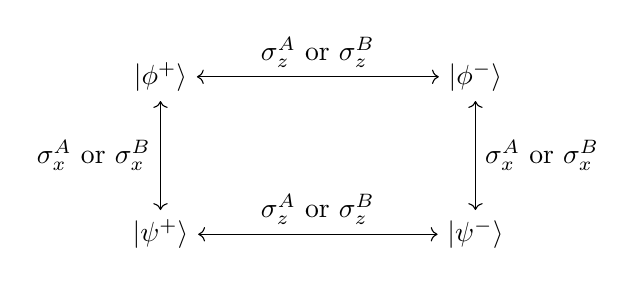
\begin{tikzpicture}
        \node[draw=none] (A) at (0,0) {$\ket{\psi^+}$};
        \node[draw=none] (B) at (0,2) {$\ket{\phi^+}$};
        \node[draw=none] (C) at (4,2) {$\ket{\phi^-}$};
        \node[draw=none] (D) at (4,0) {$\ket{\psi^-}$};

        \path [<->] (A) edge node[left] {$\sigma_x^A$ or $\sigma_x^B$} (B);
        \path [<->] (B) edge node[above] {$\sigma_z^A$ or $\sigma_z^B$} (C);
        \path [<->] (A) edge node[above] {$\sigma_z^A$ or $\sigma_z^B$} (D);
        \path [<->] (D) edge node[right] {$\sigma_x^A$ or $\sigma_x^B$} (C);
    \end{tikzpicture}
    \caption{Switching between Bell states with \text{LOOC}}
\end{figure}
\end{document}